\section{Exempelskript för ickelinjär kurvanpassning}
\label{sec:matlab-exempel}
Nedan finner ni ett Matlab skript ({\tt passning.m}) för incke linjär kurvanpassning.
Ekvationen som passas i exemplet är helt godtycklig:

\begin{equation}
  \label{eq:ex}
  f(x) = a\frac{x^b+1}{x^{b+1}+1}
\end{equation}

Vi genererar data för passning med brus och låter Matlabs funktion
``fit'' optimera $a$ och $b$ (se \cref{fig:matlab}).

\begin{figure}
  \centering
  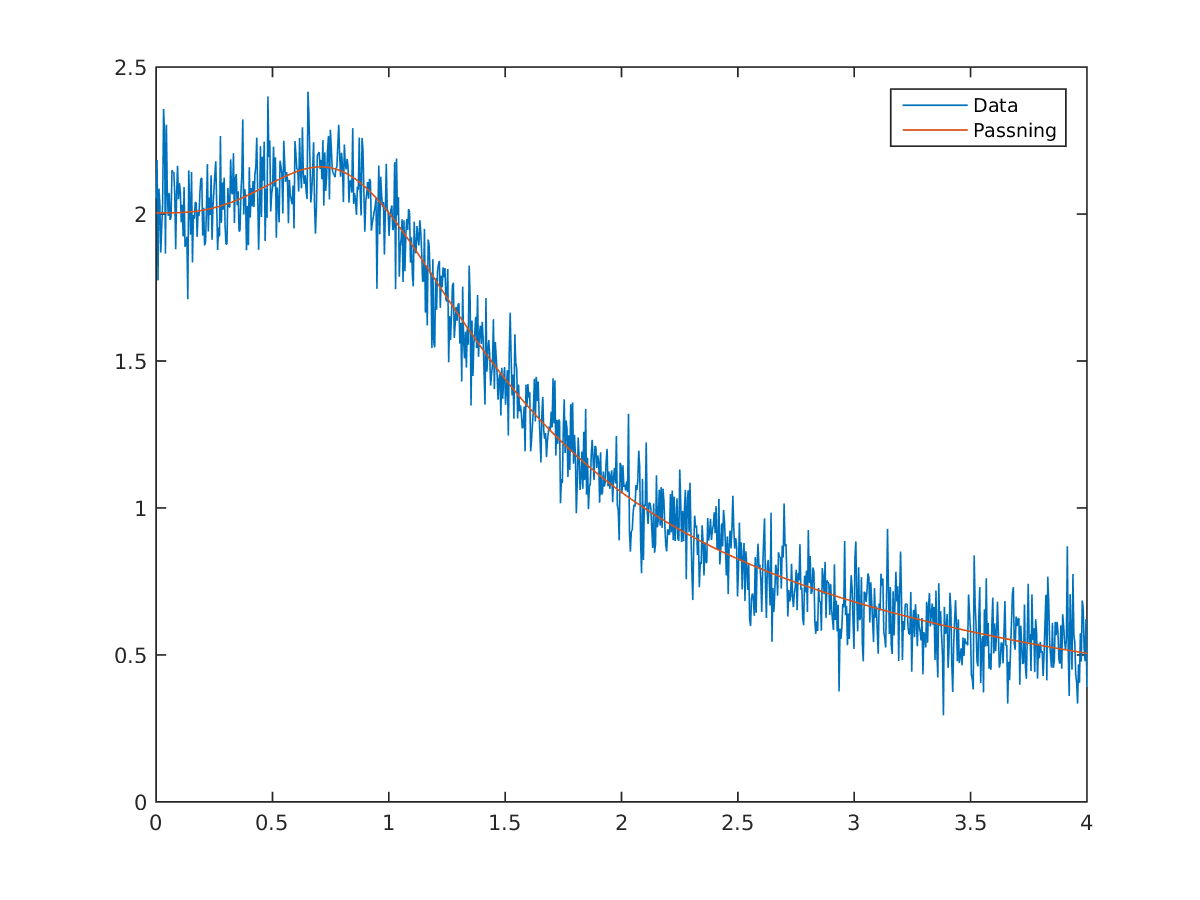
\includegraphics[scale=0.5]{matlab/passning.png}
  \caption{Ickelinjär kurvanpassning}
  \label{fig:matlab}
\end{figure}

\matlabcode{matlab/passning.m}

När vi exekverar koden ovan får vi följande utdata i terminalen:

\begin{terminaloutput}
>> passning

fitobj = 

     General model:
     fitobj(x) = (a*(x.^b+1)./(x.^(b+1)+1))
     Coefficients (with 95% confidence bounds):
       a =       2.004  (1.988, 2.02)
       b =       3.207  (2.813, 3.601)
\end{terminaloutput}

Vi ser att passningen lyckades och de sanna värdena ligger väl inom
angivna 95\%  konfidensintervall. Vi noterar dock att osäkerheten är
relativt stor för {\tt b}. Observera att vi gav startvärdena 1 för
optimeringen av $a$ och $b$. För att kurvanpassningen skall vara pålitlig
bör man försöka välja så bra startvärden som möjligt. Genom att titta på
den brusiga kurvan i \cref{fig:matlab} kunde vi t. ex. från
skärningspunkten med y-axeln satt startgissningen för $a$ någonstans
kring 2 och sedan löst ut $b$ ur en approximativ version av \cref{eq:ex} för
$f(4) \approx 0.5$.